\documentclass[twoside,leqno,twocolumn]{article}  
\usepackage{ltexpprt} 
\usepackage{amssymb,amsmath}
\usepackage{cleveref}
\usepackage{algorithm}
\usepackage{times}
\usepackage{color}
\usepackage{url}
\usepackage{subfigure}
\usepackage{xspace}
\usepackage[noend]{algorithmic}
\usepackage{enumerate}
\usepackage{multirow}
\usepackage{balance} 
\usepackage{epstopdf}
\usepackage[english]{babel}
\usepackage{graphicx}
\usepackage{enumitem}
%\usepackage{caption}
%\usepackage{subcaption}


\newcommand{\squishlist}{
   \begin{list}{$\bullet$}
    {
      \setlength{\itemsep}{0pt}
      \setlength{\parsep}{3pt}
      \setlength{\topsep}{3pt}
      \setlength{\partopsep}{0pt}
      \setlength{\leftmargin}{1.5em}
      \setlength{\labelwidth}{1em}
      \setlength{\labelsep}{0.5em} } }

\newcommand{\squishend}{
    \end{list}  }


\newcommand{\model}{{STAT}\xspace} %stat is an abbreviation for statim which means immediately in latin
\newcommand{\fullmodel}{{{\sf SourceSeer}}\xspace}
\newcommand{\locationmodel}{{\sf LocSeer}\xspace}
\newcommand{\keymodel}{{\sf KeyWord}\xspace}
\newcommand{\w}{{\bf w}}
\newcommand{\z}{{\bf z}}
\newcommand{\loc}{{\bf l}}
\newcommand{\tim}{{\bf t}}
\newcommand{\todo}[1]{\textcolor{red}{{TODO: #1}}}

\newtheorem{definition}{Definition}
\newtheorem{example}{Example}

\begin{document}

%\CopyrightYear{2007} % Allows default copyright year (20XX) to be over-ridden - IF NEED BE.
%\crdata{0-12345-67-8/90/01}  % Allows default copyright data (0-89791-88-6/97/05) to be over-ridden - IF NEED BE.
% --- End of Author Metadata ---

\title{\fullmodel: Forecasting Rare Disease Outbreaks \\ Using Multiple Data Sources - Supplementary Material}
\date{}

\author {
Theodoros Rekatsinas$^1$, Saurav Ghosh$^2$, Sumiko R. Mekaru$^3$, Elaine O. Nsoesie$^3$ \\ 
John S. Brownstein$^3$, Lise Getoor$^4$, Naren Ramakrishnan$^2$ \\
{\small \texttt{thodrek@cs.umd.edu, sauravcsvt@cs.vt.edu}}\\ 
{\small \texttt{\{sumiko.mekaru,elaine.nsoesie, john.brownstein\}@childrens.harvard.edu,}} \\
{\small \texttt{getoor@soe.ucsc.edu, naren@cs.vt.edu}}\\ 
{\small $^1$University of Maryland, $^2$Virginia Tech}
{\small $^3$Boston Children's Hospital, $^4$University of California, Santa Cruz}
}


\maketitle

\section{Gibbs Sampling for \model}
\label{sec:gibbs}
We provide the detailed derivation of the Gibbs sampling algorithm in Section 3. The joint distribution corresponding to the topic model is:
\begin{align}
&\Pr(\w,\tim,\loc,\z,{\bf \phi},{\bf \theta},{\bf \xi};\alpha,\beta,\gamma) =  \nonumber \\
&=\prod_{z = 1}^{K}\Pr(\phi_z;\beta)\Pr(\xi_z;\gamma) \prod_{l = 1}^{L}\Pr(\theta_l;\alpha) \nonumber \\
& \cdot \prod_{s = 1}^{S}\prod_{i = 1}^{N_s} \Pr(z_{si}|l_{si},\theta_l)\Pr(w_{si}|\phi_{z_{si}})\Pr(t_{si}|\xi_{z_{si}}) \nonumber
\end{align}
Next, we marginalize over all ${\bf \phi}$, ${\bf \xi}$ and ${\bf \theta}$. We have:

\begin{align}
&\Pr(\w,\tim,\loc,\z;\alpha,\beta,\gamma) \nonumber \\
&=  \int_{\phi}\int_{\theta}\int_{\xi} \Pr(\w,\tim,\loc,\z,{\bf \phi},{\bf \theta},{\bf \xi};\alpha,\beta,\gamma) d\xi d\theta d\phi \nonumber \\
&=\int_{\phi} \prod_{z = 1}^{K}\Pr(\phi_z;\beta) \prod_{s = 1}^{S}\prod_{i = 1}^{N_s}\Pr(w_{si}|\phi_{z_{si}}) d\phi \nonumber \\
& \cdot \int_{\xi} \prod_{z = 1}^{K} \Pr(\xi_z;\gamma)\prod_{s = 1}^{S}\prod_{i = 1}^{N_s}\Pr(t_{si}|\xi_{z_{si}}) d\xi \nonumber \\
&\cdot \int_{\theta} \prod_{l = 1}^{L}\Pr(\theta_l;\alpha)\prod_{s = 1}^{S}\prod_{i = 1}^{N_s}\Pr(z_{si}|l_{si},\theta_{l_{si}})d\theta \nonumber \\
&=\int_{\phi} \prod_{z = 1}^{K}\Pr(\phi_z;\beta) \prod_{s = 1}^{S}\prod_{i = 1}^{N_s}\Pr(w_{si}|\phi_{z_{si}}) d\phi \nonumber \\
&  \cdot \int_{\xi} \prod_{z = 1}^{K} \Pr(\xi_z;\gamma)\prod_{s = 1}^{S}\prod_{i = 1}^{N_s}\Pr(t_{si}|\xi_{z_{si}}) d\xi \nonumber \\
&\cdot \int_{\theta} \prod_{l = 1}^{L}\Pr(\theta_l;\alpha)\prod_{s = 1}^{S}\prod_{i = 1}^{N_s}\Pr(z_{si}|l_{si},\theta_{l_{si}}) d\theta \nonumber
\end{align}

We focus on the different integrals in the expression presented above. We start with the integral over ${\bf \phi}$. 

\begin{align}
& \int_{\phi} \prod_{z = 1}^{K}\Pr(\phi_z;\beta) \prod_{s = 1}^{S}\prod_{i = 1}^{N_s}\Pr(w_{si}|\phi_{z_{si}}) d\phi \nonumber \\
& =  \prod_{z = 1}^{K} \int_{\phi_{z}} \Pr(\phi_z;\beta) \prod_{s = 1}^{S}\prod_{i = 1}^{N_s}\Pr(w_{si}|\phi_{z_{si}}) d\phi_{z} \nonumber \\
&= \prod_{z = 1}^{K} \int_{\phi_z} \frac{\Gamma(\sum_{r = 1}^V \beta_r)}{\prod_{r = 1}^V \Gamma(\beta_r)}\prod_{r = 1}^V \phi_{zr}^{\beta_r -1} \prod_{r = 1}^V \phi_{zr}^{n^{z}_{(\cdot),r}} d\phi_z \nonumber \\
&= \prod_{z = 1}^{K} \int_{\phi_z} \frac{\Gamma(\sum_{r = 1}^V \beta_r)}{\prod_{r = 1}^V \Gamma(\beta_r)}\prod_{r = 1}^V \phi_{zr}^{\beta_r  + n^{z}_{r} -1} d\phi_z \nonumber \\
& = \prod_{z = 1}^K \frac{\Gamma(\sum_{r = 1}^V \beta_r)}{\prod_{r = 1}^V \Gamma(\beta_r)} \frac{\prod_{r = 1}^V \Gamma(n^{z}_{r} + \beta_r)}{\Gamma(\sum_{r =1}^V n^{z}_{r} + \beta_r)} \nonumber
\end{align}
where $n^{z}_{r}$ denotes the number of times word $r$ was associated with topic $z$ across all sources and entries. Similarly we have for the $\xi$ part:

\begin{align}
&\int_{\xi} \prod_{z = 1}^{K} \Pr(\xi_z;\gamma)\prod_{s = 1}^{S}\prod_{i = 1}^{N_s}\Pr(t_{si}|\xi_{z_{si}}) d\xi \nonumber \\
&= \prod_{z = 1}^K \int_{\xi_z} \Pr(\xi_z;\gamma)\prod_{s = 1}^{S}\prod_{i = 1}^{N_s}\Pr(t_{si}|\xi_{z_{si}}) d\xi \nonumber \\
& = \prod_{z = 1}^K \frac{\Gamma(\sum_{t = 1}^T \gamma_t)}{\prod_{t = 1}^T \Gamma(\gamma_t)} \frac{\prod_{t = 1}^T \Gamma(m^{z}_{t} + \gamma_t)}{\Gamma(\sum_{t =1}^T m^{z}_{t} + \gamma_t)} \nonumber
\end{align}
where $m^{z}_{t}$ denotes the number of times time-point $t$ was associated with topic $z$ across all sources. Finally, we focus on the $\theta$ integral. We follow a similar analysis and have the following:

\begin{align}
&\int_{\theta} \prod_{l = 1}^{L}\Pr(\theta_l;\alpha)\prod_{s = 1}^{S}\prod_{i = 1}^{N_s}\Pr(z_{si}|l_{si},\theta_{l_{si}}) d\theta \nonumber \\
&= \prod_{l = 1}^L \int_{\theta_l} \Pr(\theta_l;\alpha)\prod_{s = 1}^{S}\prod_{i = 1}^{N_s}\Pr(z_{si}|l_{si},\theta_{l_{si}}) d\theta_l \nonumber \\
& = \prod_{l =1}^L\int_{\theta_l} \frac{\Gamma(\sum_{z = 1}^K \alpha_z)}{\prod_{z = 1}^K \Gamma(\alpha_z)}\prod_{z = 1}^K \theta_{lz}^{\alpha_z -1}\prod_{z=1}^K\theta_{lz}^{o^z_{l}}d\theta_l \nonumber \\
&= \prod_{l =1}^L\int_{\theta_l} \frac{\Gamma(\sum_{z = 1}^K \alpha_z)}{\prod_{z = 1}^K \Gamma(\alpha_z)}\prod_{z = 1}^K \theta_{lz}^{\alpha_z  + o^z_{l}-1}d\theta_l \nonumber \\
& = \prod_{l =1}^L\frac{\Gamma(\sum_{z = 1}^K \alpha_z)}{\prod_{z = 1}^K \Gamma(\alpha_z)}\frac{\prod_{z=1}^K\Gamma(o^z_l + \alpha_z)}{\Gamma(\sum_{z = 1}^K o^z_l + \alpha_z)}\nonumber
\end{align}
where $o^z_l$ denotes the number of times location $l$ was associated with topic $z$ across all sources and their entries. 
Eventually we have that the joint distribution is given by:

\vspace{-10pt}\begin{align}
&\Pr(\w,\tim,\loc,\z;\alpha,\beta,\gamma) = \prod_{z = 1}^K \frac{\Gamma(\sum_{r = 1}^V \beta_r)}{\prod_{r = 1}^V \Gamma(\beta_r)} \frac{\prod_{r = 1}^V \Gamma(n^{z}_{r} + \beta_r)}{\Gamma(\sum_{r =1}^V n^{z}_{r} + \beta_r)} \nonumber \\
&\cdot \prod_{z = 1}^K \frac{\Gamma(\sum_{t = 1}^T \gamma_t)}{\prod_{t = 1}^T \Gamma(\gamma_t)} \frac{\prod_{t = 1}^T \Gamma(m^{z}_{t} + \gamma_t)}{\Gamma(\sum_{t =1}^T m^{z}_{t} + \gamma_t)} \nonumber \\
& \cdot \prod_{l =1}^L\frac{\Gamma(\sum_{z = 1}^K \alpha_z)}{\prod_{z = 1}^K \Gamma(\alpha_z)}\frac{\prod_{z=1}^K\Gamma(o^z_l + \alpha_z)}{\Gamma(\sum_{z = 1}^K o^z_l + \alpha_z)}  \nonumber
\end{align}
The goal of Gibbs sampling is to approximate the conditional distribution $\Pr(\z | \w, \tim,\loc;\alpha,\beta,\gamma,\Psi)$. Using the chain rule we have the following for the conditional probability:

\begin{align}
&\Pr(z_{si}| \w,\tim,\loc,\z_{-si};\alpha,\beta,\gamma) \nonumber \\
&= \frac{\Pr(z_{si}, w_{si}, t_{si}, l_{si}|\w_{-si},\tim_{-si},\loc_{-si},\z_{-si};\alpha,\beta,\gamma)}{\Pr(w_{si}, t_{si}, l_{si}|\w_{-si},\tim_{-si},\loc_{-si},\z_{-si};\alpha,\beta,\gamma)} \nonumber \\
& \propto \frac{n^{k,-(s,i)}_{w_{si}} + \beta_{w_{si}}}{\sum_{r = 1}^V n^{k,-(s,i)}_{r} + \beta_{r}} \cdot \frac{m^{k,-(s,i)}_{t_{si}} + \gamma_{t_{si}}}{\sum_{t = 1}^T m^{k,-(s,i)}_{t} + \gamma_{t}} \nonumber \\
& \cdot \frac{o^{k,-(s,i)}_{l_{si}} + \alpha_{l_{si}}}{\sum_{l = 1}^L o^{k,-(s,i)}_{l} + \alpha_{l}} \nonumber
\end{align}
where $-si$ in the superscript indicates that the current example has been excluded by the count summations. 

\section{Topic Model Evaluation for Common Diseases}
\label{sec:common_topics}

\begin{table*}[t]
\begin{center}
\caption{Three discovered topics that are related to Influenza (Avian Flu), dengue and Swine Flu. Histograms show the topic prominence over time; The top words with their probability in each topic are shown.}
\begin{tabular}{|lr|lr|lr|}
\hline
\multicolumn{2}{|c|}{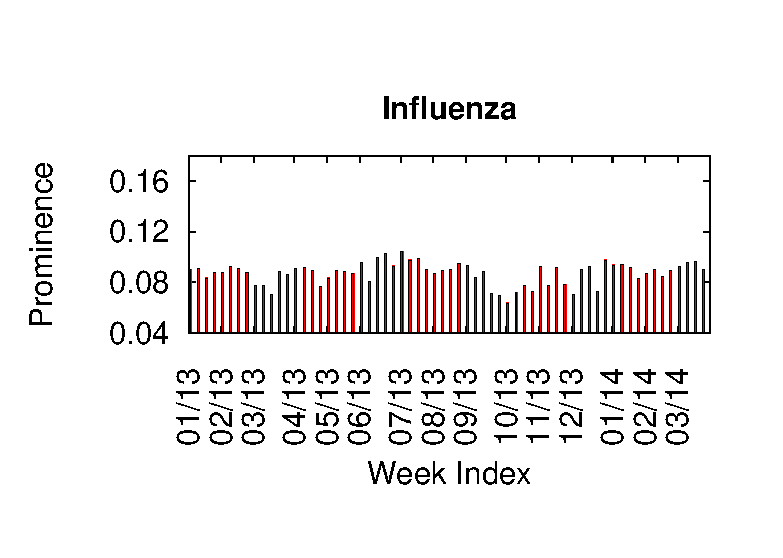
\includegraphics[clip,scale=0.45]{fig/topic_influenza_timeline.eps}} & \multicolumn{2}{|c|}{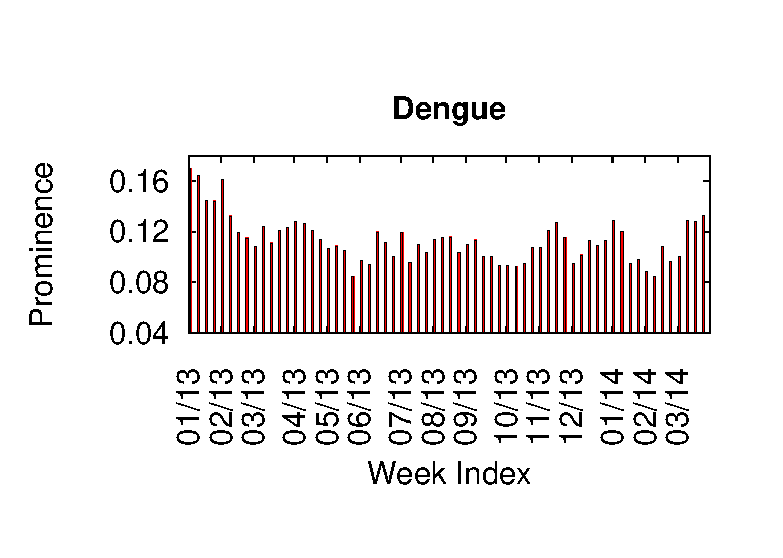
\includegraphics[clip,scale=0.45]{fig/topic_dengue_timeline.eps}}& 
\multicolumn{2}{|c|}{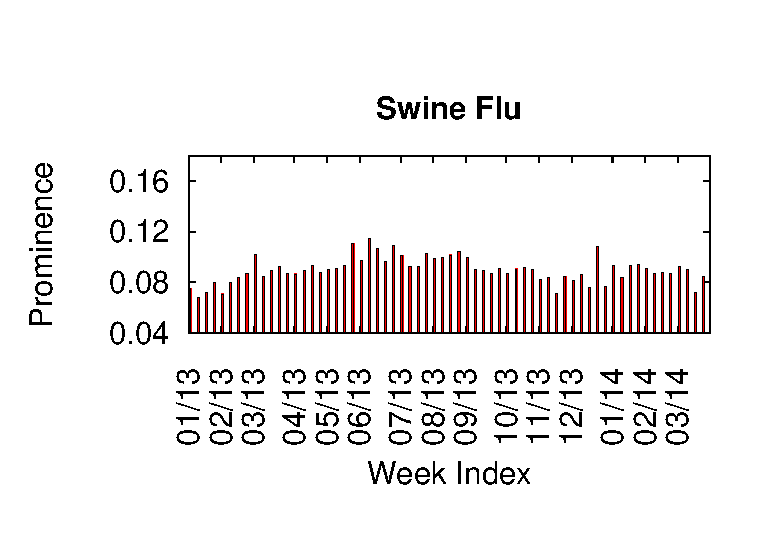
\includegraphics[clip,scale=0.45]{fig/topic_swine_timeline.eps}} \\ \hline
influenza & 0.0567 & dengue & 0.2095 & gripe & 0.0522 \\
mosquito & 0.0495 & aegypti & 0.0166 & h1n1 & 0.0351 \\
pacientes & 0.0258 & agua & 0.0137  & infectadas &0.0043 \\
aviar & 0.0144 & mosquitos & 0.0058  & flu & 0.0024\\
larvas & 0.0096 & agricultura & 0.0019 & bacteria & 0.0021 \\
fiebre & 0.0088 & respiratoria & 0.0018 & enfermo & 0.0008 \\
surto & 0.0061 & rurales & 0.0006 & vacinas & 0.0008 \\
zancudos & 0.0008 & agropecuario	 & 0.0006 & nasal & 0.0008 \\
avian & 0.0006 & hemorragias & 0.0005 & paracetamol & 0.0007 \\
h5n1 & 0.0003 & suero & 0.0004 & swine & 0.0005 \\
\hline
\end{tabular}\label{tab:common_topics}
\end{center}
\end{table*}

We evaluate the performance of the proposed topic model at discovering common disease topics and their temporal patterns. \Cref{tab:common_topics} shows three topics related to avian flu, dengue and swine flu. Again, we present their most likely words and their prominence histograms over time. For all three topics we see that the corresponding disease keywords, i.e., ``influenza",  ``dengue" and ``gripe" (flu) are ranked first. For the avian influenza topic, the proposed topic model is able to discover the correlation among words referring to both the {\em causes}, i.e., ``mosquito", ``larvas", ``zancudos" (mosquitos), and the {\em symptoms}, i.e., ``fiebre" (fever), of the disease. Regarding the dengue topic, our approach is able to identify the main transmission root of dengue which is via the aides aegypti mosquito, as well as, the fact that dengue is more prominent in rural and agricultural areas. Finally, a similar performance is observed for the swine flu topic. Our approach can identify the correlation between the word ``bacteria" and swine flu - bacteria co-infections play a key role in swine flu deaths - and the correlation between ``paracetamol" and swine flu, one of indicated medication substances for the disease.

\section{Detailed Evaluation of Different Prediction Approaches}
\label{sec:full_eval}
In this section, we present the detailed evaluation results for the performance of BSR, \keymodel, \locationmodel, and \fullmodel on predicting Hantavirus incidences from January 2013 to March 2014. \Cref{tab:results} shows the precision, recall and F1 score  of the four approaches aggregated over Chile, Argentina, Brazil and Uruguay. For \locationmodel and \fullmodel we report the results for the configuration $k$ that obtained the best performance. 

\begin{table*}[h]
 \centering
  \caption{BSR, \keymodel, \locationmodel and \fullmodel on predicting hantavirus outbreaks. Notation $(k\% )$ denotes the best performing configuration for \locationmodel and \fullmodel. }
  \begin{tabular}{|c|c|c|c|c|c|c|c|c|c|c|c|c|}
    \hline
    & \multicolumn{3}{c|}{{\bf BSR}} &
    \multicolumn{3}{c|}{{\bf \keymodel}} &
    \multicolumn{3}{c|}{{\bf \locationmodel(5\%)}} &
    \multicolumn{3}{c|}{{\bf \fullmodel(5\%)}} \\
    \cline{2-10} {\em Month}   & {\em Prec.} & {\em Rec.} & {\em F1} & {\em Prec.} & {\em Rec.} & {\em F1} & {\em Prec.} & {\em Rec.} & {\em F1} & {\em Prec.} & {\em Rec.} & {\em F1} \\
    \hline 
    01/13 & 0.5 & 0.17 & 0.25 & {\bf 0.67}& 0.33& 0.44& 0.13 & {\bf 0.67} & 0.22 & 0.44 & {\bf 0.67} & {\bf 0.53}\\ 
    \hline
     02/13 & 0.52 & 0.78 & 0.62 & {\bf 0.67} & {\bf 1.0}& {\bf 0.80} & 0.12 & {\bf 1.0} & 0.21 & 0.5 & {\bf 1.0} & 0.67\\ 
    \hline
    03/13 & {\bf 0.7} & 0.35 & 0.46 & 0.6 & {\bf 0.75} & {\bf 0.67} & 0.29 & 0.5 & 0.37 & 0.5 & 0.5 & 0.5\\ 
    \hline
    04/13 & {\bf 0.78} & 0.59 & 0.67 & 0.33  & 0.25  & 0.28 & 0.6 & 0.75 & 0.67 & 0.57 & {\bf 1.0} & {\bf 0.73}\\ 
    \hline
    05/13 & {\bf 0.51} & 0.48 & {\bf 0.54} & 0.29 & 0.4 & 0.34& 0.14 & 0.2 & 0.16 & 0.38 & {\bf 0.6} & 0.47\\ 
    \hline
    06/13 & {\bf 0.22} & 0.68 & {\bf 0.33} & 0& 0& 0& 0.14 & {\bf 1.0} & 0.25 & 0.14 & {\bf 1.0} & 0.25\\ 
    \hline
    07/13 & {\bf 0.22} & 0.68 & {\bf 0.33} & 0& 0& 0& 0.14 & {\bf 1.0} & 0.25 & 0.2 & {\bf 1.0} & {\bf 0.33}\\ 
    \hline
    08/13 & 0.4 & 0.6 & 0.47 & 0& 0& 0& 0.2 & {\bf 1.0} & 0.33 & {\bf 0.67} & {\bf 1.0} & {\bf 0.80}\\ 
    \hline
    09/13 & 0.5 & 0.33 & 0.39 & 0& 0& 0& 0.23 & {\bf 1.0} & 0.37 & {\bf 0.67} & {\bf 0.67} & {\bf 0.67}\\ 
    \hline
    10/13 & {\bf 0.62} & 0.24 & 0.35 & 0.5& 0.4& 0.44& 0.31 & {\bf 0.8} & 0.45 & 0.38 & 0.6 & {\bf 0.47}\\ 
    \hline
    11/13 & {\bf 0.89} & 0.44 & 0.59 & 0.75& 0.5& {\bf 0.6}& 0.21 & {\bf 0.83} & 0.34 & 0.45 & {\bf 0.83} & 0.58\\ 
    \hline
    12/13 & 0.9 & 0.32 & 0.47 & {\bf 0.75}& 0.27& 0.40& {\bf 0.75} & {\bf 0.55} & {\bf 0.63} & 0.67 & {\bf 0.55} & 0.60\\ 
    \hline
    01/14 & 0.65 & 0.49 & 0.56 & 0.43& 0.38& 0.40& 0.19 & 0.5 & 0.28 &  {\bf 0.71}& {\bf 0.63} & {\bf 0.67}\\ 
    \hline
    02/14 & 0.56 & {\bf 0.74} & 0.64 & 0.43 & 0.5 & 0.46 & 0.27 &  0.67 & 0.38 & {\bf 0.67} & 0.67 & {\bf 0.67}\\ 
    \hline
    03/14 & 0.55 & {\bf 0.88} & {\bf 0.68} & {\bf 0.57} & 0.8& 0.66& 0.29 & 0.8 & 0.42 & 0.5 & 0.8 & 0.62 \\ 
    \hline
  \end{tabular}
  \vspace{-10pt}
  \label{tab:results}
\end{table*}

As shown, \fullmodel  obtains the best F1-score and recall for most of the months. We observe that the recall obtained by \locationmodel is comparable to that of \fullmodel, while the recall of BSR is significantly lower compared to that of both \locationmodel and \fullmodel. The latter is expected as BSR can only predict outbreaks for states where a sufficient number of outbreaks has occurred in the past. In fact, due to its design BSR fails completely to forecast outbreaks for states or countries where no outbreaks have been observed in the past (e.g., the outbreak in Brazil for October 2013 and the outbreak in Uruguay for March 2013).  However this mechanism limits the number of false positives significantly, and thus, for many months we observe slightly higher or comparable precision scores for BSR with those of \fullmodel. On the other hand the precision scores of \locationmodel are significantly lower compared to \fullmodel. The reason for this behavior is the increased number of false positives returned by \locationmodel even after the thresholding mechanism was employed. Regarding \keymodel, we observe that the model performs reasonably well when there is an increase in the number of outbreaks in previous weeks leading to increased keyword counts. However, the model performs poorly for cases when a small number of words was observed in the previous weeks. For example \keymodel failed to forecast Hantavirus outbreaks in August  and September 2013 because only one incidence was mentioned in July. 



\end{document}
